\documentclass{beamer}
\usepackage[utf8]{inputenc}
\usepackage[T1]{fontenc}
\usepackage[francais]{babel} 
\usepackage{lmodern}
\usepackage{hyperref}
\usepackage{pgfplots}
\usepackage{tikz}
\usepackage{algorithm2e}

\usetikzlibrary{trees,shapes.geometric,arrows,decorations.pathmorphing,backgrounds,fit,positioning,shapes.symbols,chains,patterns}
 \tikzset{
    %Define standard arrow tip
    >=stealth',
    %Define style for boxes
    punkt/.style={
           rectangle, dashed,
           rounded corners,
           draw=black, very thin,
           minimum height=2em,
           minimum width = 2cm,
           text centered},
    square/.style={
           rectangle,
           draw=black, thick,
           minimum height=.5cm,
           text centered},
    data/.style={
           rectangle,
           draw=black, thick,
           minimum height= 2cm,
           minimum width = 2cm,
           text centered},
    % Define arrow style
    pil/.style={
           ->,
           thick,
           shorten <=1pt,
           shorten >=1pt,},
    asym/.style={
           <->,
           thin,
           shorten <=1pt,
           shorten >=1pt,
           red!100},
    sym/.style={
           <->,
           thin,
           shorten <=1pt,
           shorten >=1pt,
           blue!100}
}


\usetikzlibrary{shapes.gates.logic.US,trees,positioning,arrows}
\tikzstyle{startstop} = [rectangle, rounded corners, minimum width=3cm, minimum height=1cm,text centered, draw=black, fill=red!30]
\tikzstyle{io} = [trapezium, trapezium left angle=70, trapezium right angle=110, minimum width=3cm, minimum height=1cm, text centered, draw=black, fill=blue!30]
\tikzstyle{process} = [rectangle, minimum width=3cm, minimum height=1cm, text centered, draw=black, fill=orange!30]
\tikzstyle{processH} = [rectangle, minimum width=1cm, minimum height=1cm, text centered, draw=black, fill=orange!30]
\tikzstyle{processS} = [rectangle, minimum width=1.3cm, minimum height=1.3cm, text centered, draw=black, fill=orange!30]
\tikzstyle{decision} = [diamond, minimum width=3cm, minimum height=1cm, text centered, draw=black, fill=green!30]
\tikzstyle{punkt} = [rectangle, dashed, rounded corners, draw=black, very thin,minimum height=2em,minimum width = 2cm, text centered]
\tikzstyle{arrow} = [thick,->,>=stealth]



\usepackage{eurosym}
\usepackage{rotating}
\usepackage{array}
\usepackage{multicol}

\usetheme{Antibes}
\usecolortheme{beaver}
\setbeamertemplate{sections/subsections in toc}[square]
\setbeamertemplate{blocks}[square]%

\author{Claire Smets -- William Boisseleau -- Pascal Edouard -- Mathieu Latimier -- Julien Legras}
\title{Soutenance projet annuel - Audit des implantations SSL/TLS}
\titlegraphic{
\includegraphics[height=3em]{logo_univ.png}}
\institute{Master 2 Sécurité des Systèmes Informatiques}

\date{28/02/2014}

\begin{document}
{
\setbeamertemplate{headline}[default] 
\begin{frame}
  \titlepage
\end{frame}
}

%% 2 MIN -- PASCAL
\section{Introduction}
\subsection{Sujet et problématique}
\frame{
\frametitle{Sujet et problématique}
\begin{block}{Les clefs qui rôdent sur internet}
	\begin{itemize}
		\item clefs SSH (Port 22), SSL/TLS (Port 443)
		\item taille des clefs + génération aléatoire\\
	\end{itemize}
\end{block}

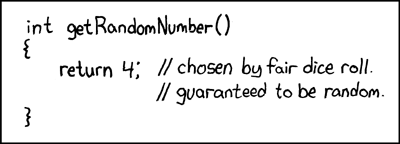
\includegraphics[height=7em]{images/random_number.png}
}

\frame{
\frametitle{Sommaire}
\begin{multicols}{2}
\tableofcontents
\end{multicols}
}

%% PARTIE 1 - 16 MIN
\section{Audit des clefs RSA des certificats}

%% 4 MIN -- CLAIRE
\subsection{Récupération}
\subsubsection{Adresses}
\frame{
    \frametitle{Récupération des adresses 1}
    	\begin{block}{ZMAP}
	\begin{itemize}
		\item open source ;
		\item outil de scan réseau ;
		\item adresses IPv4 ;
		\item paquets SYN sur le port 443.\\
	\end{itemize}
	\end{block}
}

\subsubsection{Certificats}
\frame	{
    \frametitle{Récupération des certificats 1}
    %% Certificats + clefs
    \begin{block}{Application Récupération de Certificats}
	\begin{itemize}
		\item script perl ;
		\item certificats SSL ;
		\item stocker l'ensemble des empreintes dans un dossier : 
		\begin{itemize}
			\item certificats ;
			\item clefs de session.\\
		\end{itemize}	
	\end{itemize}
	\end{block}
}

\frame{
    \frametitle{Récupération des certificats 2}
    	\begin{block}{Algorithme}
    		\tiny
			\begin{algorithm}[H]
				\label{alg:recupCertif}
				 %\SetAlgoLined % For previous releases [?]
				 \Entree{Fichier f, contenant les adresses ayant le port 443 ouvert}
				 \Sortie{Certificats et clef de session des adresses}
				 \Donnees{log, certificat, clef de session}
				 
				 \PourTous{adresses de f}{
					Se connecter au serveur\;
					\eSi{echec}{
						\Si{le log contient \textit{protocol}}{
					 		on incrémente le nombre d'échecs de protocoles\;
					 	}
					 	\Si{le log contient \textit{handshake}}{
					 		on incrémente le nombre d'échecs de poignées de mains\;
						}
					}{
					On capture la session (dont le certificat serveur)\;
					\Si{!echec de capture de session}{
						on extrait le certificat et la clef de session\;
					}	 
					}
				}
				\Retour{certificats et clés de session}
				
				\end{algorithm}
				\vspace{0.7cm}	
			\end{block}
}

\frame{
    \frametitle{Gestion des doublons 1}
	\begin{block}{Gestion des doublons}
	\begin{itemize}
		\item script perl ;
		\item si une empreinte de trouve déjà dans le dossier : on la stocke dans un autre dossier, celui des doublons ;
		\item liens symboliques.\\
	\end{itemize}
	\end{block}	
}

\frame{
    \frametitle{Gestion des doublons 2}
	\begin{block}{Algorithme gestion des doublons}
	\tiny
		\begin{algorithm}[H]
			\label{alg:clean}
			 %\SetAlgoLined % For previous releases [?]
			 \Entree{Pré-requis : Exécution de l'algorithme ssl\_collector \\
			 Création d'un dossier D contenant les certificats à traiter}
			 \Sortie{Dossiers : certs\_doublons, certs\_links; Fichier : moduli}
			 \Donnees{Certificats C; Fingerprint F; Chaîne de caractères S; Modulo M}
			 certs\_doublons $\leftarrow$ dossier\_vide\;
			 certs\_links $\leftarrow$ dossier\_vide\;
			 moduli $\leftarrow$ fichier\_vide\;
			 \PourTous{C $\in$ D}{
			 	F $\leftarrow$ \textit{fingerprint}(C)\;
			 	S $\leftarrow$ \textit{nom\_fichier}(C)\;
			 	M $\leftarrow$ \textit{modulo}(C)\;
			 	\Si{échec(F)}{
			 		continue\;
			 	}
			 	\eSi{F $\in$ certs\_links}{
			 		certs\_doublons/F $\leftarrow$ concat(certs\_doublons/F, S)\;
			 	}{
			 		moduli $\leftarrow$ concat(moduli, M)\;
			 		certs\_links $\leftarrow$ F\;
			 	}
			 }
		\end{algorithm}
		\vspace{0.7cm}
	\end{block}	
}

%% 5 MIN
% julien et william
\subsection{Factorisation}
\frame{
    \frametitle{Factorisation}
    \framesubtitle{PGCD deux à deux}
\begin{center}
\begin{tikzpicture}
\begin{scope}[node distance=1cm,on grid,>=stealth',
		block/.style={rectangle,draw,fill=cyan!20},
		comp/.style={circle,draw,fill=orange!40},
		block2/.style={rectangle,draw,fill=orange!40}]	
		

	\node [block2] (N1)		[] {$N_1$};
	\node [block2] (N2)		[right=of N1,xshift=1.2cm] {$N_2$} ;
	\node [block2] (N3)		[right=of N2,xshift=1.2cm] {$N_3$} ;
	\node [block2] (N4)		[right=of N3,xshift=1.2cm] {$N_4$}  ;\pause	
	
	\node [block2] (N21) [below=of N1,xshift=+1.8cm] {$N_1N_2$} edge [<-] (N1) edge [<-] (N2) ;	
	\node [block2] (N22) [right=of N21,xshift=2cm] {$N_3N_4$} edge [<-] (N3) edge [<-] (N4) ;	\pause

	\node [block2] (P) [below=of N21,xshift=1.4cm] {$N_1N_2N_3N_4$} edge [<-] (N21) edge [<-] (N22);\pause
	
	\node [block2] (mod1) [below=of P,xshift=-1.4cm] {$\mod (N_1N_2)^2$}  edge [<-] (P); 
	\node [block2] (mod2) [right=of mod1,xshift=2cm] {$\mod (N_3N_4)^2$}  edge [<-] (P);\pause
	
	\node [block2] (mod21)		[below=of mod1,xshift=-1.8cm] {$\mod N_1^2$} edge [<-] (mod1);
	\node [block2] (mod22)		[right=of mod21,xshift=1.2cm] {$\mod N_2^2$} edge [<-] (mod1);
	\node [block2] (mod23)		[right=of mod22,xshift=1.2cm] {$\mod N_3^2$}  edge [<-] (mod2);
	\node [block2] (mod24)		[right=of mod23,xshift=1.2cm] {$\mod N_4^2$}  edge [<-] (mod2);\pause

	
	\node [block2] (div1)		[below=of mod21] {$/N_1$} edge [<-] (mod21);
	\node [block2] (div2)		[below=of mod22] {$/N_2$} edge [<-] (mod22);
	\node [block2] (div3)		[below=of mod23] {$/N_3$}  edge [<-] (mod23);
	\node [block2] (div4)		[below=of mod24] {$/N_4$}  edge [<-] (mod24);\pause

	\node	[block2]	(gcd1)	[below=of div1]	{$pgcd(.,N_1)$} edge [<-] (div1);
	\node	[block2]	(gcd2) [below=of div2]		{$pgcd(.,N_2)$} edge [<-] (div2);
	\node	[block2]	(gcd3) [below=of div3]		{$pgcd(.,N_3)$} edge [<-] (div3);
	\node	[block2]	(gcd4) [below=of div4]	 	{$pgcd(.,N_4)$} edge [<-] (div4);\pause
\end{scope}

\end{tikzpicture}

\end{center}
}


\frame{
    \frametitle{Factorisation}
    \framesubtitle{Exemple}

\begin{center}
\begin{tikzpicture}[scale=0.9, every node/.style={scale=0.9}]
\begin{scope}[node distance=1cm,on grid,>=stealth',
		node/.style={transform shape},
		block/.style={rectangle,draw,fill=cyan!20},
		comp/.style={circle,draw,fill=orange!40},
		block2/.style={rectangle,draw,fill=orange!40}]	
		

	\node [block2] (N1)		[] {$2*3$};
	\node [block2] (N2)		[right=of N1,xshift=1.2cm] {$3*5$} ;
	\node [block2] (N3)		[right=of N2,xshift=1.2cm] {$7*11$} ;
	\node [block2] (N4)		[right=of N3,xshift=1.2cm] {$1$}  ;\pause	
	
	\node [block2] (N21) [below=of N1,xshift=+1.8cm] {$90$} edge [<-] (N1) edge [<-] (N2) ;	
	\node [block2] (N22) [right=of N21,xshift=2cm] {$70$} edge [<-] (N3) edge [<-] (N4) ;	\pause

	\node [block2] (P) [below=of N21,xshift=1.4cm] {$6930$} edge [<-] (N21) edge [<-] (N22);\pause
	
	\node [block2] (mod1) [below=of P,xshift=-3.2cm] {$\mod (90)^2 = 6930$}  edge [<-] (P); 
	\node [block2] (mod2) [below=of P,xshift=3.2cm] {$\mod (70)^2 = 1001$}  edge [<-] (P);\pause
	
	\node [block2] (mod21)		[below=of mod1,xshift=-1.5cm] {$\mod 6^2 = 18$} edge [<-] (mod1);
	\node [block2] (mod22)		[below=of mod1,xshift=1.5cm] {$\mod 15^2 = 180$} edge [<-] (mod1);
	\node [block2] (mod23)		[below=of mod2,xshift=-1.5cm] {$\mod 77^2 = 1001$}  edge [<-] (mod2);
	\node [block2] (mod24)		[below=of mod2,xshift=1.5cm] {$\mod 1^2 = -$}  edge [<-] (mod2);\pause

	
	\node [block2] (div1)		[below=of mod21] {$/6=3$} edge [<-] (mod21);
	\node [block2] (div2)		[below=of mod22] {$/15=12$} edge [<-] (mod22);
	\node [block2] (div3)		[below=of mod23] {$/77=13$}  edge [<-] (mod23);
	\node [block2] (div4)		[below=of mod24] {$-$}  edge [<-] (mod24);\pause
	
	\node	[block2]	(gcd1) [below=of div1]	{$pgcd(3,6)=3$} edge [<-] (div1);
	\node	[block2]	(gcd2) [below=of div2]		{$pgcd(12,15)=3$} edge [<-] (div2);
	\node	[block2]	(gcd3) [below=of div3]		{$pgcd(13,77)=1$} edge [<-] (div3);
	\node	[block2]	(gcd4) [below=of div4]	 	{$-$} edge [<-] (div4);\pause
\end{scope}

\end{tikzpicture}

\end{center}
}


\frame{
    \frametitle{Factorisation}
    \framesubtitle{Algorithmes associés : Arbre des produits, Arbre des restes}
    
    \begin{columns}
    		\begin{column}{.48\textwidth}

\begin{algorithm}[H]
 \scriptsize
 \Entree{tableau des moduli : T}
 \Sortie{Hauteur arbre, produits des moduli\\}
 
 $v \leftarrow T$\;
 $level \leftarrow 0$\;
 \Tq{$|v|>1$}{
  $tmp \leftarrow \emptyset$\;
  \PourCh{$i \in \{0, .., |v| / 2\}$}{
    $tmp[i] \leftarrow v[i\times2] \times v[i\times2 + 1]$\;
  }
  $storeProductLevel(v, level)$\;
  $v \leftarrow tmp$\;
  $level \leftarrow level + 1$\;
 }
 \Retour{level}

\end{algorithm}


    		\end{column}
    		\hfill
    		
    		\begin{column}{.48\textwidth}


\begin{algorithm}[H]
 \scriptsize
 \Entree{Hauteur de l'arbre : level}
 \Sortie{PGCDs des moduli}
 \Tq{$level>0$}{
  $P \leftarrow getRemainderLevel(level)$\;
  $v \leftarrow getProductLevel(level-1)$\;
  \PourCh{$i \in \{0, .., |v|\}$}{
    $v[i] \leftarrow P[i/2] \pmod{v[i]^2}$\;
  }
  $storeRemainderLevel(v, level)$\;
  $v \leftarrow tmp$\;
  $level \leftarrow level - 1$\; 
 }
 $w \leftarrow \emptyset$\;
 \PourCh{$i \in \{0, .., |v|\}$}{
    $w[i] \leftarrow P[i/2] \pmod{v[i]^2}$\;
    $w[i] \leftarrow w[i] / v[i]$\;
    $w[i] \leftarrow pgcd(w[i],v[i])$\;
  }
 \Retour{w}

\end{algorithm}

    		\end{column}  
    \end{columns}


}



\frame{
    \frametitle{Factorisation -- Démonstration}

}

%% 5 MIN -- PASCAL
\subsection{Résultats}
\frame{
    \frametitle{Résultats}
\begin{block}{Base de donnée}
   	\begin{itemize}
		\item Récupération des facteurs communs - clefs publique
		\item Scripts perl + requêtes SQL \\
	\end{itemize}
\end{block}

\begin{block}{Statistiques}
   	\begin{itemize}
		\item Les émetteurs
		\item Outil de recherche
		\begin{itemize}
			\item taille de clef : 99.6\% (R) - 0.4\% (V)
			\item émetteurs, sujet : CISCO - 6280 (R) - 40 (V)\\
		\end{itemize}
	\end{itemize}
\end{block}
}


%% PARTIE 2 - 16 MIN
\section{Audit d'OpenSSL}
\frame{
%% 1 MIN -- CLAIRE
\frametitle{Introduction}
	\begin{block}{Contexte}
	\begin{itemize}
		\item récent scandal sur la NSA ;
		\item beaucoup d'outils utilisés. \\
	\end{itemize}
	Mais à qui peut-on faire confiance?
	\end{block}
	\begin{block}{Audit d'OpenSSL}
		Cinq grands axes : 
		\begin{itemize}
			\item l'entropie ;
			\item la génération des clefs ;
			\item le chiffrement et les protocoles ;
			\item les signatures et les authentifications ;
			\item les protocoles SSL et TLS.\\
		\end{itemize}
	\end{block}
}

\frame{
\frametitle{Failles}
	\begin{block}{Où ?}
		\begin{itemize}
			\item site des CVE ;
			\item site de Vigil@nce ;
			\item RFC.\\
		\end{itemize}
	\end{block}
	
	\begin{block}{Quand ?}
		\begin{itemize}
			\item année passée ;
			\item failles plus anciennes.
		\end{itemize}
	\end{block}
	
	\begin{block}{Corrections ?}
		Présence de corrections? Si oui, lesquelles et par qui?
	\end{block}
}

%% 4 MIN -- WILLIAM (3 MIN)
\subsection{Entropie}
\subsection{Entropie}
\frame{
\frametitle{Entropie}
\framesubtitle{Définitions}


\begin{block}{Générateur}
\begin{itemize}

\item problème aléatoire ;
\item mesure de l'entropie $H(X) = - \sum_x P(X=x)*\log_2(P(X=x))	 $ ;
\item entropie et moduli.

\end{itemize}
\end{block}
	
}


\frame{
\frametitle{Entropie}

\begin{center}
\begin{tikzpicture}[scale=0.75, every node/.style={scale=0.75},node distance=1.5cm]
\node (donnees) [io,pattern=dots,pattern color=orange] {Données};
\node (digit) [process, right of=donnees, xshift=4cm] {Digitalisation};
\node (cond) [process, below of=digit,text width=3cm,yshift=-0.5cm] {Conditionnement (optionnel)};
\node (bat) [process, right of=cond, xshift=4cm] {Batterie de tests}; 
\node (dec) [decision, below of=cond,yshift=-1.2cm] {Sortie}; 
\node (appli) [process, below of=dec, yshift=-1cm] {Application};

\begin{pgfonlayer}{background}
\node[punkt, fit=(donnees)(digit)(cond)(bat)(dec), fill=yellow!5] (groupclient) {};
\end{pgfonlayer}

\begin{pgfonlayer}{background}
\node[punkt, fit=(donnees)(digit), fill=yellow!20] (groupclient) {};
\end{pgfonlayer}

\draw [arrow] (donnees) -- (digit);
\draw [arrow] (digit) -- node[anchor=east] {out1}(cond);
\draw [arrow] (cond) -- node[anchor=east] {out2} (dec);
\draw [arrow] (digit) -| node[anchor=south] {out1} (bat);
\draw [arrow] (cond) -- node[anchor=south] {out2} (bat);
\draw [arrow] (bat) |- node[anchor=north] {true/false} (dec);
\draw [arrow] (dec) -- node[anchor=east] {output/error} (appli);
\end{tikzpicture}
\end{center}
}


\frame{
\frametitle{Entropie}

\begin{block}{Tests}
\begin{itemize}
\item Tests trop anciens, \texttt{FIPS1} (1994), non mis à jour
 	\begin{itemize}
 	\item test monobit
	\item test poker
	\item test runs
	\item test long runs
	\end{itemize} 	 
\item Autres tests proposés dans le rapport

\end{itemize}
\end{block}
		
	
}


%% MATHIEU (1 MIN)
\frame{
\frametitle{Entropie -- Démonstration}
\begin{block}{Faille Debian 4.0 sous OpenSSL 0.9.8}
Après avoir récupéré l'ensemble des certificats sur l'Internet, on peut identifier rapidement ceux qui ont étés générés durant la faille Debian/OpenSSL entre 2006 et 2008.\\
\begin{itemize}
\item \textbf{Durée de l'attaque} : quelques heures
\item \textbf{Conséquences} : forger de faux certificats, de fausses signatures et déchiffrer des messages privées.
\item \textbf{Qui?} : grandes entreprises (e.g. IBM, CISCO), routeurs, universités, etc.
\item \textbf{Fin de validité de certificats} : Entre 2020 et 2030.
\end{itemize}
\end{block}
}

%% 2 MIN -- MATHIEU
\subsection{Génération des clefs}
\frame{
\frametitle{Génération des clefs}
\begin{block}{Principes de Kerchkoff}
	\begin{itemize}
	\item Le \textit{secret} réside dans la clef ;
	\item Les algorithmes de génération de clés ne doivent donner aucune information sur la clé.
	\end{itemize}
\end{block}

\begin{block}{Deux grands types de générateur de clés}
\begin{itemize}
\item Générateurs de bits aléatoires (RGB) pour les clés privées de certains algorithmes (i.e. AES, DSA) ou pour le salage (i.e. \textit{seed} de RSA)
\item Générateurs de clefs asymétriques, qui utilisent des fonctions à sens uniques, largement diffusées et ne devant délivrer aucune information sur le secret.
\end{itemize}
\end{block}
}

\frame{
\frametitle{Génération des clefs}
\begin{block}{Audit : Diffie-Hellman Ephémère en mode FIPS}
\begin{itemize}
\item \textbf{Description} : Un attaquant écoutant une communication chiffré en SSL/TLS entre un client et un serveur peut déchiffrer tout les messages en forçant la génération d'un secret Diffie-Hellman prédictible.
\item \textbf{Comment?} : En modifiant le trafic réseau par exemple.
\item \textbf{Pourquoi?} : L'activation du mode FIPS ne rejette pas les paramètres P/Q faibles pour les algorithmes EDH/DHE.
\item \textbf{Où?} : Dans \texttt{crypto/dh/dh\_key.c} une partie de code génère un faux positif dans certains cas (sur une condition de test).
\item \textbf{Solution :} Logiciel \textit{Nessus Vulnerability Scanner} pour tester la configuration des serveurs.
\end{itemize}
\end{block}
}

%% 2 MIN -- CLAIRE
\subsection{Chiffrement et protocoles}
\frame{
\frametitle{Chiffrement et protocoles}

}

%% 2 MIN -- MATHIEU
\subsection{Signature et authentification}
\frame{
\frametitle{Signature et authentification}
\begin{block}{Définition}
\begin{itemize}
\item Juridiquement, une signature électronique à même valeur qu'une signature manuscrite.
\item Elle \textbf{DOIT} assurer l'intégrité, l'authentification et la non-répudiation d'un message.
\end{itemize}
\end{block}

Des anciennes versions d'OpenSSL ont des vulnérabilités au niveau de la vérification de messages signés, ou des fuites d'informations sur la clé privée ayant servi à chiffrer.
}

\frame{
\frametitle{Signature et authentification}
\begin{block}{Audit : Attaque par injection de fautes sur les certificats RSA.}
\begin{itemize}
\item \textbf{Description} : L'attaque se fait sur des morceaux de la signature récupéré afin de récupérer la clé privée bit à bit.
\item \textbf{Comment?} : Du bon matériel, surtout au niveau de la mémoire vive (i.e. Système Linux avec une architecture SPARC) et un oracle (e.g. système de prédictions) permettant de fabriquer la clé.
\item \textbf{Temps de l'attaque} : une centaine d'heure.
\end{itemize}
\end{block}
}

\frame{
\frametitle{Signature et authentification}
\begin{block}{Audit : Attaque par injection de fautes sur les certificats RSA.} 
\begin{itemize}
\item \textbf{Un problème dans le code OpenSSL?} : La fonction \texttt{Fixed\_Window\_Exponentiation} utilise des milliers de multiplications, qui est opération la plus sensible en cas de dégradation du micro-processeur.
\item \textbf{Solution :} Aucune! On pourrait utiliser la technique du \texttt{square\_and\_multiply} mais elle a l'inconvénient d'être vulnérable à une attaque par \textit{timing}.
\item \textbf{Conséquences :} A moins que l'attaquant n'ai accès physiquement à votre machine les risques sont faibles. Cependant l'Université du Michigan cherche un moyen de faire des injections à distance à base d'\texttt{impulsions lasers}.
\end{itemize}
\end{block}
}

%% 3 MIN -- JULIEN
\subsection{Protocole SSL/TLS}
\frame{
\frametitle{Protocole SSL/TLS}

}

%% 2 MIN -- CLAIRE
\subsection{Ouverture}
\frame{
\frametitle{Ouverture}

}


%% PARTIE 3  - 8 MIN
\section{Analyse dynamique du navigateur client}
%% 2 MIN 30 -- WILLIAM
\subsection{Faiblesses identifiées}
\frame{
\frametitle{Faiblesses identifiées}
\begin{block}{Critères}
\begin{itemize}
\item version du protocole
\item \textit{ciphersuites} proposées par le client 
\item courbes elliptiques supportées 
\item algorithmes de signature 
\item compression TLS
\item activation ou non du ticket de session
\end{itemize}
\end{block}
}




%% 2 MIN 30 --  JULIEN
\subsection{Implémentation}
\frame{
\frametitle{Implémentation}

}

%% 3 MIN -- MATHIEU
\subsection{Démonstration}
\frame{
\frametitle{Démonstration}
\begin{block}{Analyse de la sécurité des navigateurs clients}
\begin{itemize}
%% Chrome
\item Sous le navigateur graphique \texttt{Chrome} : le plus utilisé dans le monde.
%% Lynx  
\item Sous le navigateur console \texttt{lynx} : apprécié chez les développeurs.\newline
\end{itemize}
\end{block}

\begin{block}{Modification manuelle}
Nous pouvons modifier la \textit{ciphersuite} du client avec la commande \texttt{s\_client}.
\end{block}
}

%% 2 MIN -- PASCAL
\section{Conclusion}
\frame{
\frametitle{Conclusion}
\begin{block}{Bilan}
	\begin{itemize}
		\item Mise en évidence des clefs faibles
		\item Évolution du code OpenSSL\\
	\end{itemize}
\end{block}
}
\end{document}
